\documentclass[doc,floatsintext,natbib]{apa7}
\usepackage[english]{babel}
\usepackage[utf8]{inputenc}
\usepackage{amsmath}
\usepackage{graphicx}
\usepackage{subcaption}
\usepackage{doi}
\usepackage{booktabs}
%\usepackage[dvipsnames]{xcolor}
\usepackage{placeins}
\usepackage{enumitem}
\usepackage{xcolor}
\usepackage{setspace} % for adjusting line spread
\usepackage{hyperref} 

\renewcommand{\doitext}{} % prevents superfluous addition of "doi:" in references
\renewcommand{\thefootnote}{\fnsymbol{footnote}} % uses symbols instead of numbers for footnotes
\usepackage[colorinlistoftodos, textsize=footnotesize]{todonotes}
%%\todo[inline, color=green!40]{This is a green inline comment.}

\linespread{1.3}


\title{One Model May Not Fit All: Subgroup Detection Using Model-Based Recursive Partitioning}
\shorttitle{shorttitle}
\authorsnames{Marjolein Fokkema$^1$ \& Carolin Strobl$^2$}
\authorsaffiliations{$^1$Leiden University, $^2$Universit\"at Z\"urich}

\abstract{Model-based recursive partitioning \cite{ZeilyHoth08} is a flexible framework for detecting subgroups with differential effects in a wide range of parametric models. It provides a versatile tool for detecting and explaining heterogeneity of intervention effects. In this tutorial paper, we provide an introduction to the general MOB framework. In two specific case studies, we show how MOB-based methods can be used to detect and explain heterogeneity in two widely-used frameworks in educational studies: mixed-effects and item-response theory models. In the first case study, we show how GLMM trees \cite{FokkySmit18} can be used to detect subgroups with different parameters in mixed-effects models. We apply GLMM trees to a dataset from a study of \cite{Demi09}, who compared longitudinal performance of siblings who did, and siblings who did not participate in the Head Start program. Using GLMM trees, we identify subgroups of families in which children show comparatively larger or smaller gains in performance following participation in Head Start. In a second case study, we show how Rasch trees \cite{StroyKopf15} can be used to detect subgroups with different parameters in IRT models. We show how a recently developed stopping criterion \cite{HennyDeba23} can be used to guide subgroup detection based on effect sizes instead of statistical significance.\\}

\usepackage{Sweave}
\begin{document}
\input{MOB_paper-concordance}
\renewenvironment{Schunk}{\small}{}


\maketitle



\todo[inline]{Target journal: \textit{Journal of School Psychology}. This Special Issue is on "Conceptual and Methodological Advances for Understanding Contextual, Identity, and Cultural Effects in Intervention Research". Submission deadline: October 31, 2023}


\newpage
\section{Introduction}
\label{sec:Introduction}

\todo[inline]{Introduce and explain MOB.}


\todo[inline]{\textbf{Previous Papers on IRT and Rasch Models in Journal of School Psychology}

Rasch and IRT models are often mentioned in this journal's papers as being used for scoring school assessments (e.g., Virginia Standards of Learning Assessments;  Oregon Assessment of Knowledge and Skills; Peabody individual achievement test, \cite{Luth92}).

A general introduction to IRT in the journal is provided by \cite{AnthyDiPe16}. There are also papers describing extensions to mixure IRT models \cite{AyalySant17} and many-facet Rasch measurement (MFRM) approaches that allow controlling for rater effects \cite{StycyAntr21}. 

\cite{Mall97} assessed DIF by comparing Rasch model item difficulties of WISC-III subtests between 110 severely and profoundly deaf children, 110 matched nonreferred hearing children, and the WISC-III standardization sample (N = 2,200).}



\newpage
\section{Tutorial: Subgroup Detection in Mixed-Effects Models}
\label{sec:TutorialMixed}



\subsection{Dataset}

To illustrate the use of GLMM trees, we analyze a dataset from \cite{Demi09}, who evaluated long-term benefits of participation in Head Start. Head Start is a federally funded nationwide pre-school program for children from low-income families. \cite{Demi09} compared performance of siblings who differed in their participation in the program using data from the National Longitudinal Survey of Youth (NLSY; REF). 

The sample consists of 273 families with at least two children where at least one child participated in Head Start and at least one child did not participate in Head Start or any other preschool program. Data from children in those families who participated in another preschool program were excluded. As such, siblings who did not participate in Head Start serve as a natural control to assess the effects of participating in Head Start. As the outcome variable, we take the Peabody Picture Vocabulary Test (PPVT; REF) and model PPVT trajectories over time. As the timing metric, we took the square root of the child's age in years, which yielded a pattern of approximately linear increases over time.

Our dataset contains five family characteristics: The mother's score on the Armed Forced Qualification Test (AFTQ), adjusted for age; the families' income (averaged over the years for which data was available); race (Black, Hispanic or White); mother's years of completed education; mother's height. Note that the latter variable is one that should be completely irrelevant for predicting performance on a vocabulary test; it is included here to illustrate that the GLMM tree algorithm can fruitfully distinguish signal from noise variables. The dataset comprises data from families and children for whom complete data was available. 

We load the data and inspect the first rows:

\begin{Schunk}
\begin{Sinput}
 HS_dat <- readRDS("HS_dat.Rda")
 head(HS_dat, 3)
\end{Sinput}
\begin{Soutput}
       AFTQ     Race   Income Mom_height Mom_edu_yrs ChildID MotherID Program
1  3.478122 Hispanic 37731.07        502          12   20502      205      HS
2  3.478122 Hispanic 37731.07        502          12   20501      205    None
3 15.964368    Black 16119.13        504          10   22403      224    None
  PPVT      Age
1   18 2.000000
2   48 2.645751
3   69 2.645751
\end{Soutput}
\end{Schunk}

We inspect the complete dataset by plotting PPVT scores against age, separated by program participation: None (black) versus Head Start (red). To show the effect of age and Head Start participation, we fitted a mixed-effects model comprising their main and interaction effects. To account for the correlation between repeated assessments on the same child, we specified a random intercept. The results are presented in Figure~\ref{fig:global_lmm}, which shows that children participating in Head Start show slightly higher performance than their non-participating siblings and that this difference persists over time. This result agrees with the findings of \cite{Demi09}.

\begin{figure}%
\caption{}
\begin{subfigure}{.7\textwidth}
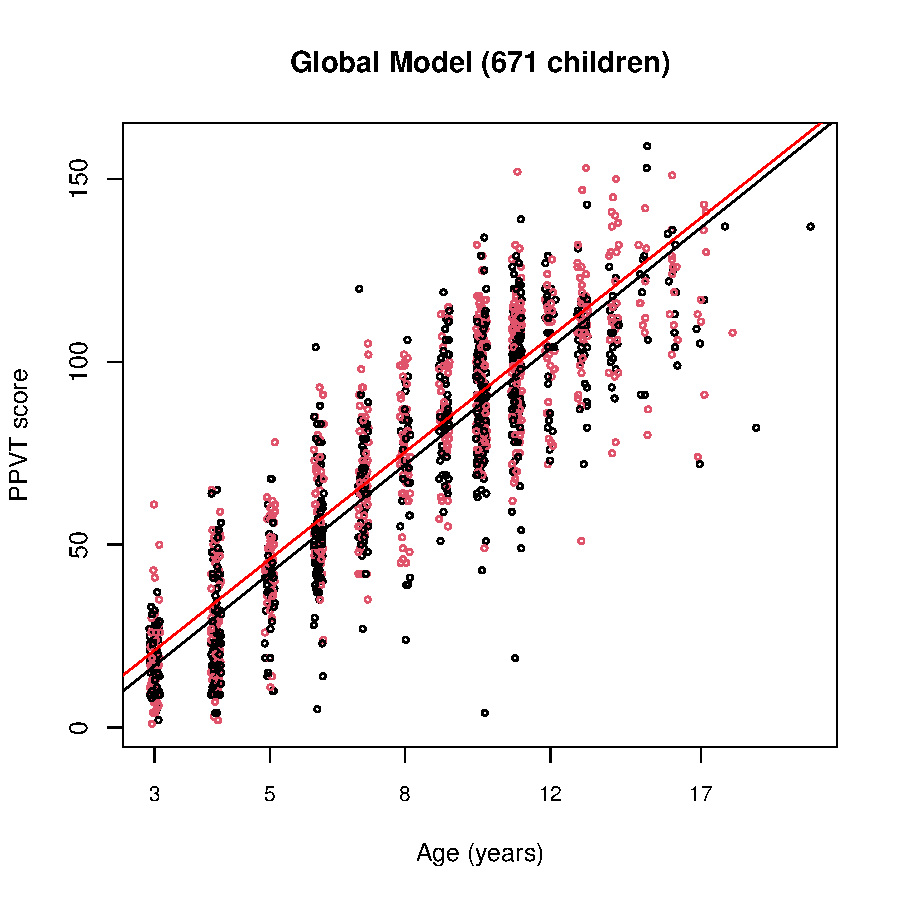
\includegraphics{MOB_paper-004}
\end{subfigure}
\label{fig:global_lmm}
\end{figure}%


\FloatBarrier
\subsection{Linear mixed effects model tree}

We now test whether the intercepts and slopes of the two regression lines differ as a function of the partitioning variables, using function \verb|lmertree| from R package \textbf{glmertree}:

\begin{Schunk}
\begin{Sinput}
 library("glmertree")
 HS_tree <- lmertree(PPVT ~ Program*Age | (1|ChildID) | AFTQ + Race + 
                       Income + Mom_edu_yrs + Mom_height, 
                     data = HS_dat, cluster = ChildID, minsize = 250)
\end{Sinput}
\end{Schunk}

With the first argument, we specified the model \verb|formula|, which has three parts separated by vertical bars: The left part (\verb|PPVT ~ Program*Age|) specifies the response variable, followed by a tilde (\verb|~|) and the fixed-effects predictors of relevance. The middle part (\texttt{1|ChildID}) specified the random effects. The right part (\verb|AFTQ + Race + Income + Mom_edu_yrs + Mom_height|) specified the partitioning variables: covariates that may possibly affect the values of the fixed-effects parameters. 

With the second argument, we specified the dataset which contain the variables. Because we are dealing with repeated measurements on the same children, we additionally specified that the parameter stability tests should be performed on the child level using the \verb|cluster| argument. Using the default observation-level parameter stability tests may artificially inflate power. Finally, because we want to retain large enough subgroups, we specified that the minimum number of observations in a terminal node should be 250.

Next, we plot the tree. With multiple fixed-effects predictors of interest, the default plots may become too crowded or difficult to interpret. We therefore specify \verb|type = "simple"| to facilitate interpretation, and using the \verb|nodesize_level| argument, we specified that the sample size printed above every terminal node should count the number of children, not the number of individual observations:

\begin{Schunk}
\begin{Sinput}
 plot(HS_tree, type = "simple", nodesize_level = 2)
\end{Sinput}
\end{Schunk}

\begin{figure}%
\caption{}
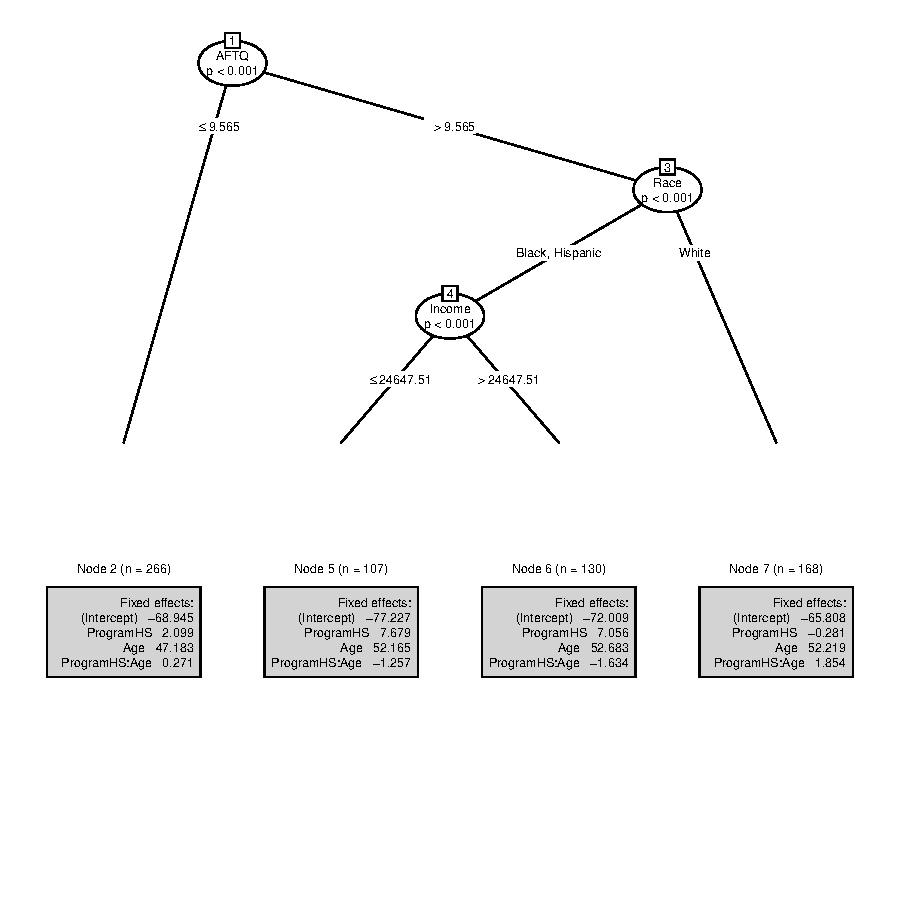
\includegraphics{MOB_paper-007}

\vspace*{-3cm}

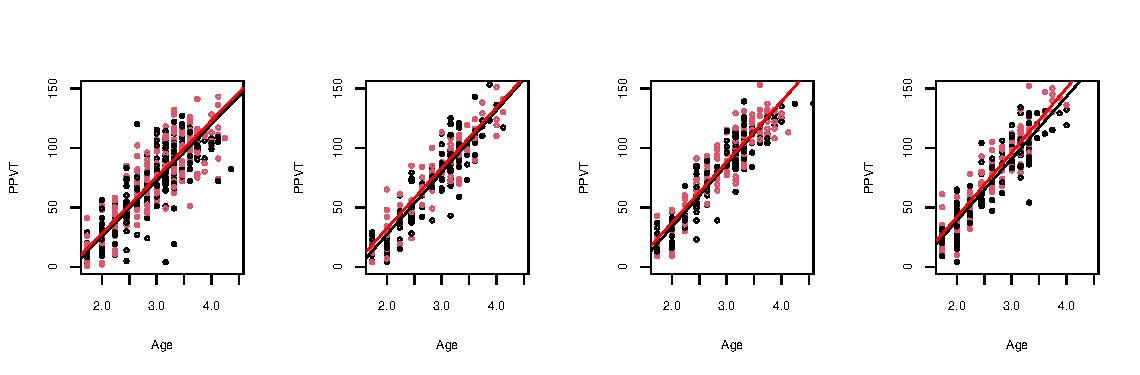
\includegraphics{MOB_paper-008}
\label{fig:lmm_tree}
\end{figure}%

The resulting tree is presented in Figure~\ref{fig:lmm_tree}. Below each terminal node, we plotted the observations and the two regression curves given by the coefficients in that node. The first split was made based on the AFTQ variable, which represents the mother's score on the Armed Forced Qualification Test, adjusted for the age at which they completed the test. The group with higher mother's AFTQ scores is further split based on race. The Black and Hispanic group is further split based on income. 

\begin{table}

\caption{\label{tab:predictions}Predicted PPVT scores at different ages.}
\begin{tabular}[t]{cccc}
\toprule
Node & Program & PPVT at age 6 & PPVT at age 18\\
\midrule
2 & None & 46.63 & 131.23\\
2 & HS & 49.39 & 134.48\\
5 & None & 50.55 & 144.09\\
5 & HS & 55.15 & 146.43\\
6 & None & 57.04 & 151.51\\
6 & HS & 60.09 & 151.63\\
7 & None & 62.10 & 155.74\\
7 & HS & 66.36 & 163.32\\
\bottomrule
\end{tabular}
\end{table}
To aid interpretation of the coefficients in Figure~\ref{fig:lmm_tree}, Table~\ref{tab:predictions} provides predicted PPVT scores for each of the groups and programs at ages 6 and 18. All nodes show a modest benefit of Head Start participation at age 6, about 3-4 points on the PPVT. This benefit remains the same over time for the group with lower mother's AFTQ scores. The benefit increases over time for White children with higher mother's AFTQ scores. Strikingly, the benefit decreases over time for Black and Hispanic children with higher mother's AFTQ scores. These results correspond to the conclusions of \cite{Demi09}. 

To evaluate whether the detected subgroups indeed contribute to better predictions, we used cross validation. We separated the 258 families in the dataset into ten equally-sized folds. We took nine of the ten folds as a training dataset on which we fitted two models: an LMM tree (i.e., an LMM with subgroups) and an LMM without subgroups (comprising main and interaction effects of age and Head Start participation, and a random intercept with respect to child). We evaluated performance on the remaining folds, by computing and evaluating accuracy of the predictions. \todo{explain MSE and $R^2$} We repeated this procedure ten times, so that all folds were used as a test set once. The results are presented in Table~\ref{tab:performance}, which shows that LMM trees generalize well: They provide better predictive accuracy compared to LMMs, while implementing only few splits. 





\begin{table}

\caption{\label{tab:performance}Cross-validated performance of LMMs and LMM trees.}
\begin{tabular}[t]{ccccc}
\toprule
method & MSE & SD & number.of.splits & R2\\
\midrule
LMM tree & 221.022 & 55.727 & 2.7 & 0.813\\
LMM & 258.233 & 71.451 & NA & 0.781\\
\bottomrule
\end{tabular}
\end{table}


\todo[inline]{I am not sure this dataset is the best GLMM tree illustration, because visualized differences between subgroups are very small and perhaps the fixed-effect part is already too complex. Alternative: Do not focus on effect of Head Start, but use as partitioning variable. Then can also use data from more families (HS or none not needed), partition using child-level characteristics, and  model specification becomes simpler.}



\newpage
\FloatBarrier
\section{Tutorial: Subgroup Detection in Rasch Models}
\label{sec:TutorialRasch}

Using Rasch trees, we assess DIF for items on math and reading \todo{decide on subscale(s) to include} from the Self-Description Questionnaire \cite{Boyl94}. We use a dataset from the Early Childhood Longitudinal Study-Kindergarten class of 1998--1999 \citep[ECLS-K; ][]{NCES10}. Data were collected from 1,018 schools across the USA. Assessments took place from kindergarten through 8th grade. Here we focus on the 8th grade assessment, in which four SDQ-II items were administered to assess perceived interest and competence in reading, and another four to assess perceived interest and competence in math. Items are presented in Appendix~\ref{sec:AppendixA}. The items were rated by the children on a 4-point scale (“not at all true” through “very true”). We coded responses 1 and 2 as 0, and responses 3 and 4 as 1, to allow for fitting a Rasch model, which assumes binary responses. 


We used three covariates as possible partitioning variables: Gender (1=Male; 2=Female), race (8 categories: 1=White, non-Hispanic; 2=Black or African-American, non-Hispanic; 3=Hispanic, race specified; 4=Hispanic, race not specified; 5=Asian; 6=Native Hawaiian or other Pasific Islander; 7= American Indian or Alaska native; 7=More than one race) and socio-economic status (range $-$5 to 3). \todo{Add more partitioning variables? This does increase number of splits. But could add one that should not have an effect, e.g., month of birth.} We analyze observations of children with complete data only, yielding a total sample size of 7,417.


We load the data and inspect the first three rows as follows:

\begin{Schunk}
\begin{Sinput}
 SDQ_dat <- readRDS("ECLSK_SDQ.Rda")
 head(SDQ_dat, 3)
\end{Sinput}
\begin{Soutput}
   C7MTHBST C7ANGRY C7LIKRD C7WRYTST C7MTHGD C7LONLY C7ENGBST C7SAD C7LIKMTH
2         4       4       4        2       4       2        4     3        4
10        4       1       4        2       4       1        4     1        4
16        3       3       1        2       3       1        4     1        4
   C7WRYWEL C7ENJRD C7WRYFIN C7ENJMTH C7WRYHNG C7GRDENG C7ASHAME GENDER RACE
2         4       4        4        3        2        3        4      2    1
10        1       3        1        4        1        4        1      2    1
16        2       1        2        4        1        4        1      1    1
   WKSESL T6INTERN T6EXTERN T6INTERP T6CONTRO
2    1.56     1.50     1.00      4.0     3.75
10   1.41     1.25     1.50      4.0     4.00
16  -2.93     1.50     2.33      2.8     3.00
\end{Soutput}
\end{Schunk}

To fit Rasch trees, we use function \verb|raschtree| which is available from R package \textbf{psychotree}. However, the stopping criterion based on the Mantel–Haenszel effect size measure is implemented in R package \verb|raschtreeMH|, which we therefore use here. \todo{might be nice to implement the MH effect-size criterion in the psychotree package for this paper, currently it seems to interfere with plotting the tree}. It can be installed and loaded as follows:

\begin{Schunk}
\begin{Sinput}
 devtools::install_github("mirka-henninger/raschtreeMH")
 library("raschtreeMH")
\end{Sinput}
\end{Schunk}


To fit a Rasch tree, we first create a \verb|data.frame| that contains the item responses and possible partitioning variables:

\begin{Schunk}
\begin{Sinput}
 math_items <- c("C7MTHBST", "C7MTHGD", "C7LIKMTH", "C7ENJMTH")
 part_vars <- c("GENDER", "RACE", "WKSESL")
 mydata <- SDQ_dat[ , part_vars]
 mydata$resp <- sapply(SDQ_dat[ , math_items], function(x) ifelse(x > 2, 1, 0)) 
\end{Sinput}
\end{Schunk}

Next, we apply function \verb|raschtree| and plot the result:

\begin{Schunk}
\begin{Sinput}
 stop_fun <- stopfun_mantelhaenszel(purification = "iterative", stopcrit = "C")
 math_tree <- raschtree(resp ~ ., data = mydata, stopfun = stop_fun)
\end{Sinput}
\end{Schunk}

\begin{Schunk}
\begin{Sinput}
 plot(read_tree, gp = gpar(cex = .7))
\end{Sinput}
\end{Schunk}

The resulting tree is presented in Figure~\ref{fig:math_tree}. The splitting nodes show the $p$-value of the corresponding parameter stability tests. The terminal depict the node-specific item difficulties. The difficulties of items 1 (C7MTHBST: Math is one of my best subjects) and 3 (C7LIKMTH: I like math) appear relatively stable and show average difficulty in every subgroup. The difficulties of items 2 (C7MTHGD: I get good grades in math) and 4 (C7ENJMTH: I enjoy doing work in math) are always lower and higher, respectively, and also seem to vary more strongly. 



\begin{figure}%
\caption{Rasch tree for the four math items.}
\begin{subfigure}{1.25\textwidth}
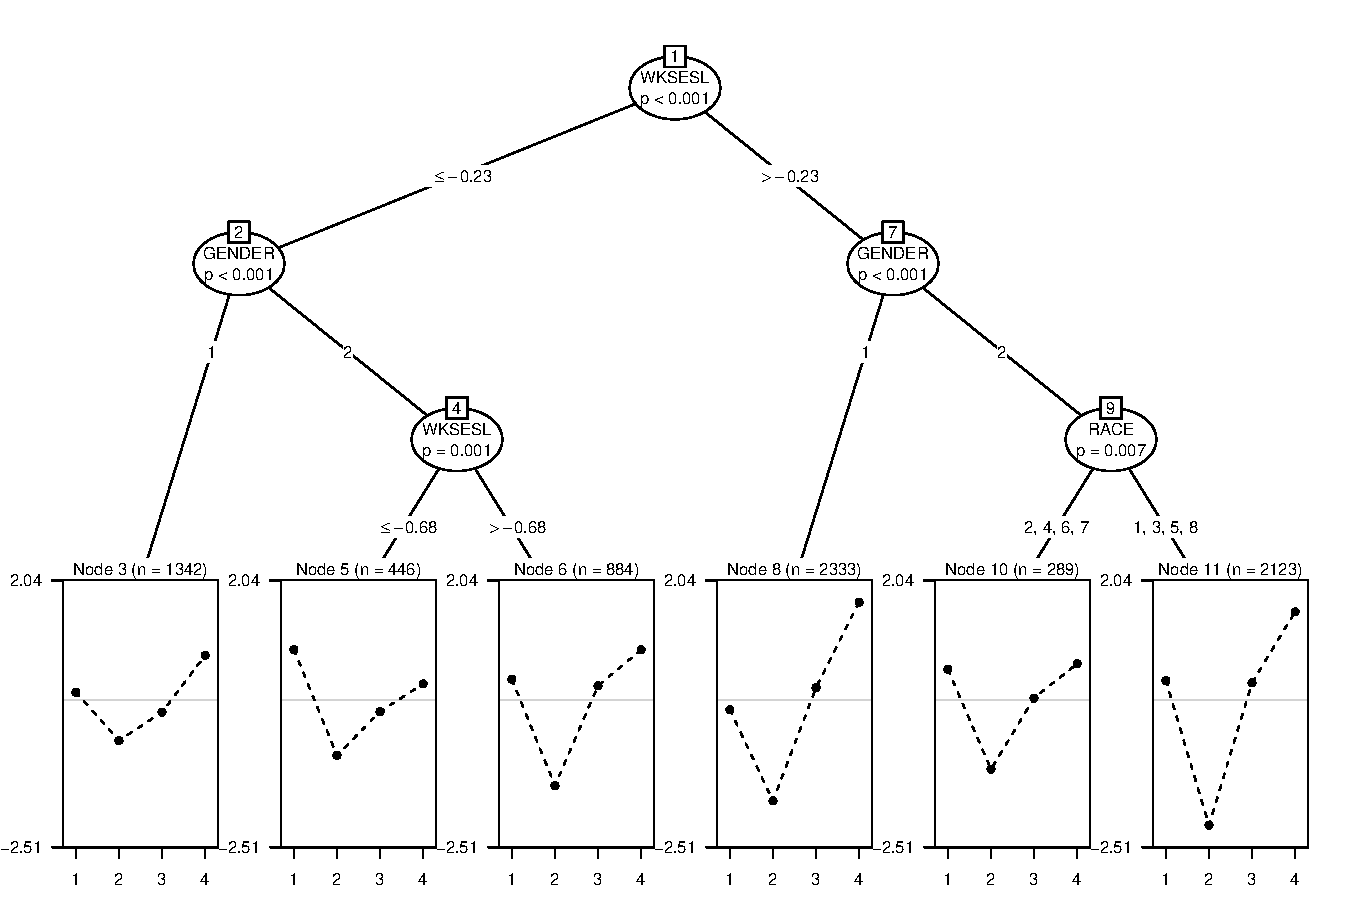
\includegraphics{MOB_paper-018}
\end{subfigure}
\label{fig:math_tree}
\end{figure}%

We repeat the procedure for the reading items:

\begin{Schunk}
\begin{Sinput}
 read_items <-  c("C7ENGBST", "C7GRDENG", "C7LIKRD", "C7ENJRD")
 mydata$resp <- sapply(SDQ_dat[ , read_items], function(x) ifelse(x > 2, 1, 0))
 read_tree <- raschtree(resp ~ ., data = mydata, stopfun = stop_fun)
\end{Sinput}
\end{Schunk}

\begin{Schunk}
\begin{Sinput}
 plot(read_tree, gp = gpar(cex = .7))
\end{Sinput}
\end{Schunk}

The resulting tree is presented in Figure~\ref{fig:read_tree}, which reveals a pattern of difficulties and splits quite similar to Figure~\ref{fig:math_tree}.

\begin{figure}%
\caption{Rasch tree for the four reading items.}
\begin{subfigure}{1.25\textwidth}
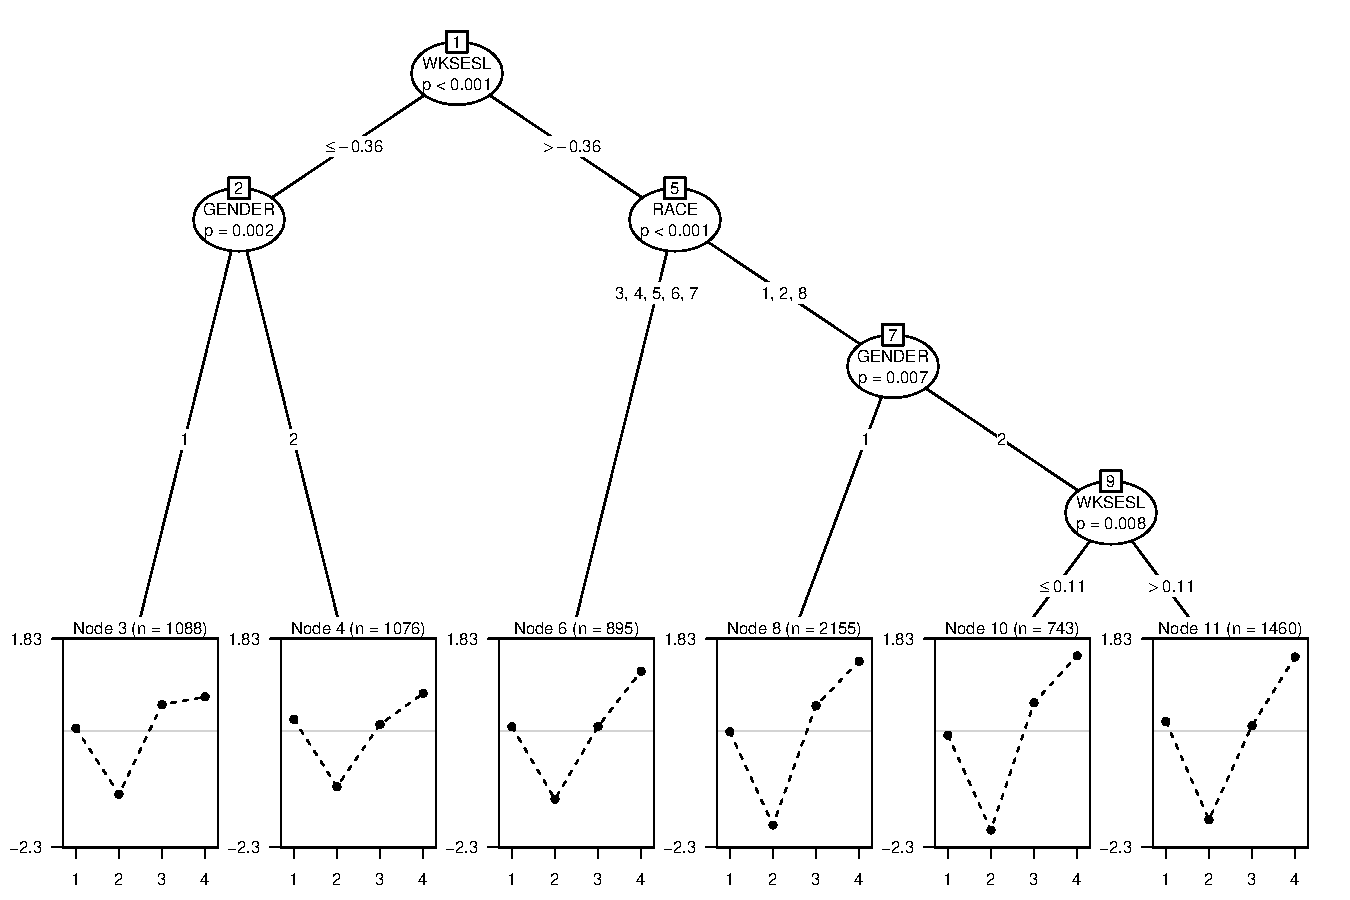
\includegraphics{MOB_paper-021}
\end{subfigure}
\label{fig:read_tree}
\end{figure}




\FloatBarrier
\section{Discussion}

\todo[inline]{Write summary of findings.}

\todo[inline]{Mention shortcomings.}

\todo[inline]{Write about future work.}







\bibliography{MOB_paper}

\todo{Add DOIs.}

\newpage
\appendix



\section{Appendix A: SDQ-II items administered in the ECLS}
\label{sec:AppendixA}

\todo{Fix formatting.}

How true is each of these about you? (1="not at all true"; 2="a little bit true"; 3="mostly true" or 4="very true")

\begin{itemize}

  \item C7MTHBST (math): Math is one of my best subjects.

  \item C7ANGRY (internalizing): I feel angry when I have trouble learning.

  \item C7LIKRD (reading): I like reading.

  \item C7WRYTST (internalizing): I worry about taking tests.

  \item C7MTHGD (math): I get good grades in math.

  \item C7LONLY (internalizing): I often feel lonely.

  \item C7ENGBST (reading): English is one of my best subjects.

  \item C7SAD (internalizing): I feel sad a lot of the time.

  \item C7LIKMTH (math): I like math.

  \item C7WRYWEL (internalizing): I worry about doing well in school.

  \item C7ENJRD (reading): I enjoy doing work in reading.

  \item C7WRYFIN (internalizing): I worry about finishing my work.

  \item C7ENJMTH (math): I enjoy doing work in math.

  \item C7WRYHNG (internalizing): I worry about having someone to hang out with at school.

  \item C7GRDENG (reading): I get good grades in English.

  \item C7ASHAME (internalizing): I feel ashamed when I make mistakes at school.

\end{itemize}


\end{document}
